
\documentclass[a4paper,12pt]{article}

\usepackage{graphicx} % Required for inserting images
\usepackage{amsmath,amssymb,amsfonts}
\usepackage{subcaption}
% -----------------------
% Package Imports
% -----------------------

% Set page margins
\usepackage[a4paper, top=1in, bottom=0.8in, left=1.1in, right=0.8in]{geometry}

% Use Times New Roman font
\usepackage{times}

% Add page numbering
\pagestyle{plain}

% Enable graphics inclusion
\usepackage{graphicx}
\usepackage{float}
% Enable code listings
\usepackage{listings}
\usepackage{xcolor} % For customizing code colors
\setlength{\parindent}{0pt}
\usepackage{physics}



\begin{document}
	\section{Experiment No. 8}
	
	\section{Experiment Title }
Determinations of Transformer Equivalent Circuit Parameters.
	\section{Objective}
	
	The objectives of this lab are as follows:
	\begin{itemize}
	 \item To perform the open-circuit and short-circuit tests on a transformer.
	\item To determine the equivalent circuit parameters of a transformer.
	\end{itemize}
	
	\section{Theory}
	\subsection{The Equivalent Circuit of a Transformer}
	
	The losses that occur in real transformers must be accounted for in any accurate model. The major items to consider in the construction of such a model are:
	
	\begin{enumerate}
		\item \textbf{Copper (I\(^2\)R) losses:} These are resistive heating losses in the primary and secondary windings of the transformer, proportional to the square of the current in the windings.
		\item \textbf{Eddy current losses:} These are resistive heating losses in the core of the transformer, proportional to the square of the voltage applied.
		\item \textbf{Hysteresis losses:} Associated with the rearrangement of magnetic domains in the core during each half-cycle, hysteresis losses are a complex, nonlinear function of the applied voltage.
		\item \textbf{Leakage flux:} The fluxes $\Phi_{LP}$ and $\Phi_{LS}$ that escape the core and pass through only one of the transformer windings are leakage fluxes. These produce self-inductance in the primary and secondary coils, which must be accounted for.
	\end{enumerate}
	
	
	\subsection{Transformer Model}
	
	It is possible to experimentally determine the values of the inductances and resistances in the transformer model. These values can be approximated using two tests: the open-circuit test and the short-circuit test.
		\subsubsection{Open-Circuit Test}
	In the open-circuit test, the transformer's secondary winding is open-circuited, and its primary winding is connected to a full-rated line voltage.Under these conditions, all the input current flows through the excitation branch of the transformer. The series elements $R_p$ and $X_p$ are too small compared to $R_c$ and $X_M$ to cause a significant voltage drop, so essentially all the input voltage is dropped across the excitation branch.
	
	 Full line voltage is applied to the primary of the transformer, and the input voltage, input current, and input power to the transformer are measured. From these measurements, it is possible to determine the power factor of the input current, which provides the magnitude and angle of the excitation impedance.
	
	The easiest way to calculate the values of $R_c$ and $X_M$ is by first looking at the admittance of the excitation branch. The conductance of the core-loss resistor is given by:
	\[
	G_C = \frac{1}{R_c}
	\]
	
	The susceptance of the magnetizing inductor is given by:
	\[
	B_M = -\frac{1}{X_M}
	\]
	
	
	The excitation admittance, $Y_E$, can be expressed as:
	\[
	Y_E = G_C - j B_M
	\]
	where $G_C$ is the conductance of the core-loss resistor, and $B_M$ is the susceptance of the magnetizing inductor.
	
	The magnitude of the excitation admittance (referred to the primary circuit) can be found from the open-circuit test voltage and current:
	\[
	|Y_E| = \frac{I_{\text{oc}}}{V_{\text{oc}}}
	\]
	where $I_{\text{oc}}$ and $V_{\text{oc}}$ are the open-circuit test current and voltage, respectively.
	
	The angle of the admittance can be found from the knowledge of the circuit power factor. The open-circuit power factor $(P_f)$ is given by:
	\[
	P_f = \cos(\theta) = \frac{P_{\text{oc}}}{V_{\text{oc}}I_{\text{oc}}}
	\]
	and the power-factor angle $\theta$ is given by:
	\[
	\theta = \cos^{-1}(P_f)
	\]
	
	The power factor is always lagging for a real transformer, so the angle of the current always lags the angle of the voltage by $\theta$ degrees. Therefore, the admittance $Y_E$ is given by:
	\[
	Y_E = \frac{V_{\text{oc}}}{I_{\text{oc}}} \angle -\theta
	\]
	where \[
	\theta = \cos^{-1}(P_f)
	\]
	
	By comparing Equations, it is possible to determine the values of $R_c$ and $X_M$ directly from the open-circuit test data.
	
	\newpage
	\subsubsection{Short-Circuit Test}
	
	In the short-circuit test, the secondary terminals of the transformer are short-circuited, and the primary terminals are connected to a fairly low-voltage source. The input voltage is adjusted until the current in the short-circuited windings reaches its rated value. It is important to ensure that the primary voltage remains at a safe level, as applying excessive voltage could damage the transformer's windings during the test.
	
	During the test, the input voltage, current, and power are measured. These values are then used to determine the parameters of the transformer's equivalent circuit, similar to the process in the open-circuit test.
	
	Since the input voltage is so low during the short-circuit test, negligible current flows through the excitation branch. If the excitation current is ignored, then all the voltage drop in the transformer can be attributed to the series elements in the circuit. The magnitude of the series impedances, referred to the primary side of the transformer, can be calculated using the measured values of voltage and current during the short-circuit test.
	
	The series impedance $Z_s$ can be expressed as:
	\[
	|Z_s| = \frac{V_{\text{sc}}}{I_{\text{sc}}}
	\]
	where \( V_{\text{sc}} \) is the input voltage during the short-circuit test, and \( I_{\text{sc}} \) is the current measured during the test.
	The short-circuit power factor $(P_f)$ is given by:
	\[
	P_f = \cos(\theta) = \frac{P_{\text{sc}}}{V_{\text{sc}}I_{\text{sc}}}
	\]
	and the power-factor angle $\theta$ is given by:
	\[
	\theta = \cos^{-1}(P_f)
	\]
	This impedance can be further split into its real and imaginary components, representing the series resistance $R_s$ and reactance $X_s$, respectively:
	\[
	Z_s = R_s + j X_s
	\]
	The values of $R_s$ and $X_s$ are determined from the magnitude of the impedance and the power factor measured during the short-circuit test.
	\newpage
	\section{Required Apparatus}
	\begin{enumerate}
		\item \textbf{Transformer}
		\begin{enumerate}
			\item Power (\(P\)): 760 VA
			\item Primary Voltage (\(U_1\)): 230 V
			\item Secondary Voltage (\(U_2\)): 400 -- 230 V
			\item Frequency (\(f\)): 50 Hz
			\item Primary Current (\(i_1\)): 3.7 A
			\item Secondary Current (\(i_2\)): 1 -- 1.7 A
		\end{enumerate}
		\item \textbf{Voltmeter:} 500 V AC rms MAX
		\item \textbf{Ammeter:} 5 A MAX
		\item Digital Multimeter Display
		\item Connecting Wires
	\end{enumerate}
	

	\section{Circuit Diagrram}

	
	\begin{figure}[H]
		\centering
		\begin{subfigure}[t]{1\textwidth}
			\centering
			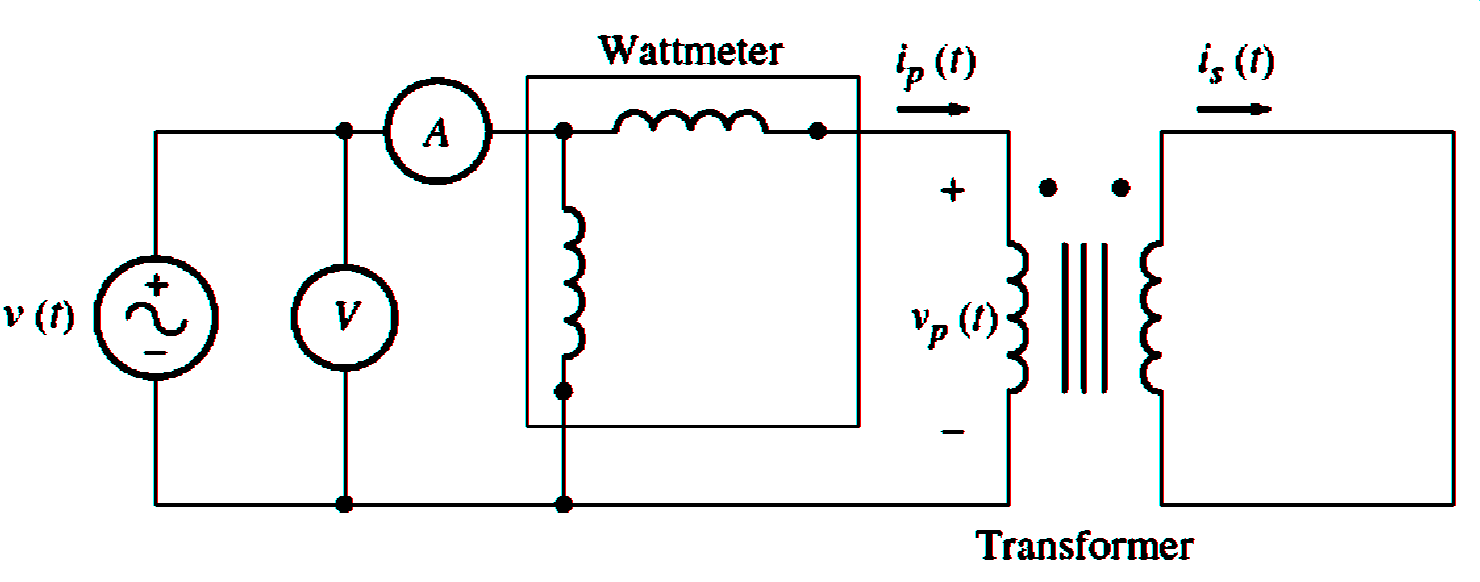
\includegraphics[width=0.8\linewidth]{Images/sc}
			\caption{Connection for transformer short-circuit test.}
			\vspace{0.5cm}
		\end{subfigure}
		
		\begin{subfigure}[t]{1\textwidth}
			\centering
			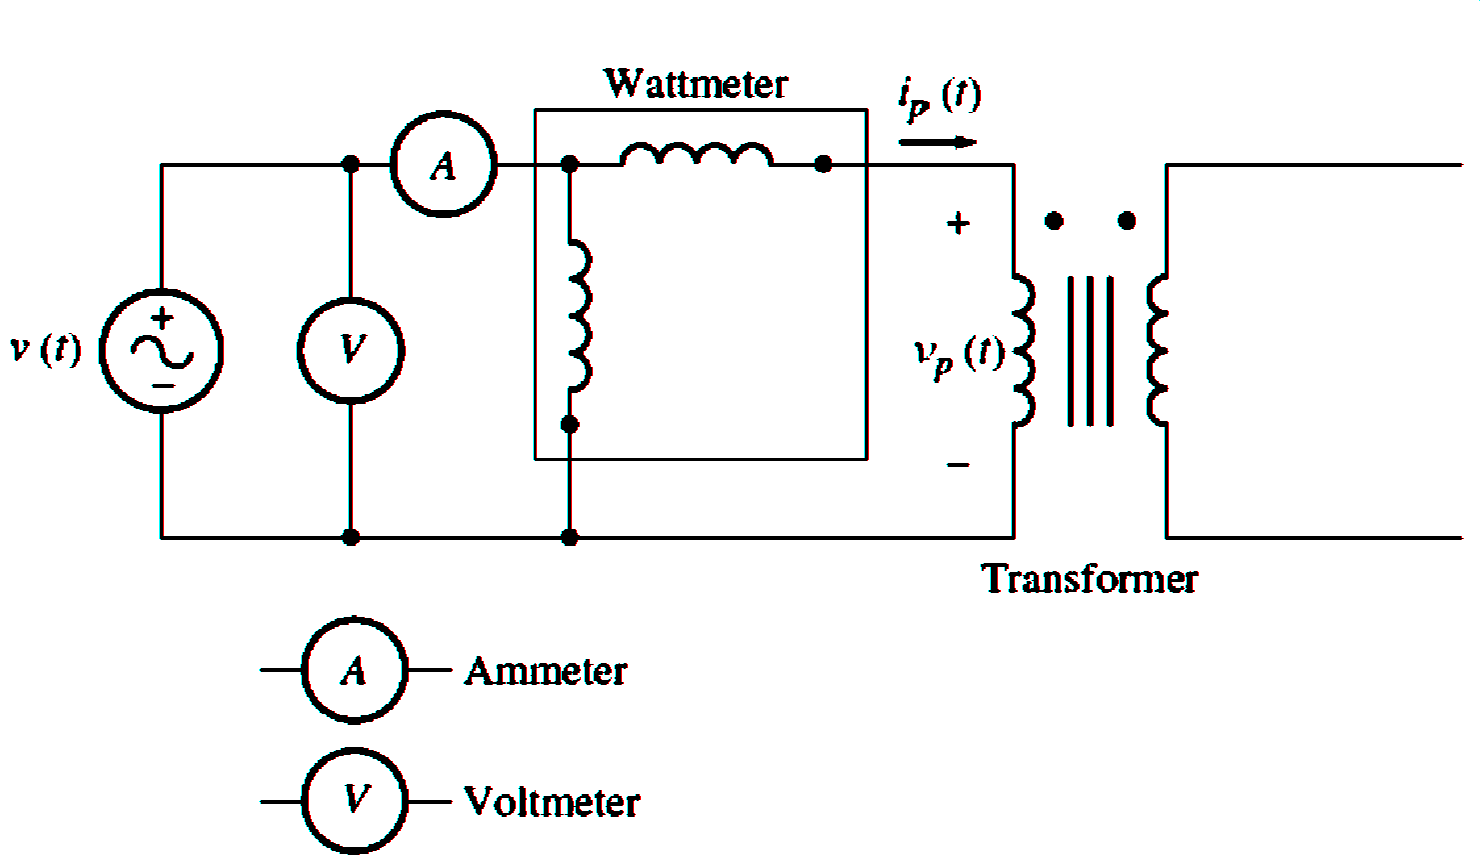
\includegraphics[width=0.75\linewidth]{Images/oc}
			\caption{ Connection for transformer open-circuit test. }
		\end{subfigure}
		
		
	\end{figure}
	
	
	\newpage
	
	
	\section{Data Table}
	\begin{table}[H]
		\caption{Table for Short Circuit Test}
		\centering
		\begin{tabular}{|c|c|c|c|c|c|c|c|c|}
			\hline
			\textbf{\begin{tabular}[c]{@{}c@{}}SI\\ No.\end{tabular}} & \textbf{\begin{tabular}[c]{@{}c@{}}Voltage,\\ $V (V)$\end{tabular}} & \textbf{\begin{tabular}[c]{@{}c@{}}Current,\\ $I(A)$\end{tabular}} & \textbf{\begin{tabular}[c]{@{}c@{}}Power,\\ $P(W)$\end{tabular}} & \textbf{\begin{tabular}[c]{@{}c@{}}Power \\ factor,\\ $P_f$ \end{tabular}} & \textbf{\begin{tabular}[c]{@{}c@{}} $\abs{Z} = \frac{V}{A}$  \end{tabular}} & $\theta= cos^{-1}(P_f) $ & \textbf{\begin{tabular}[c]{@{}c@{}}$R_s,$\\ $\Omega$ \end{tabular}} & \textbf{\begin{tabular}[c]{@{}c@{}} $X_s,$\\ $\Omega$\end{tabular}} \\ \hline
			1.                                                        & 19.7                                                              & 3.74                                                             & 72.9                                                           & 0.991                                                                    & 5.267                                                     & 7.69                           & 5.22                                                                          & 0.705                                                                         \\ \hline
		\end{tabular}
	\end{table}
	
	
	\begin{table}[H]
		\caption{Table for Open Circuit Test}
		\centering
		\scalebox{.85}{
		\begin{tabular}{|c|c|c|c|c|c|c|c|c|}
			\hline
			\textbf{\begin{tabular}[c]{@{}c@{}}SI\\ No.\end{tabular}} & \textbf{\begin{tabular}[c]{@{}c@{}}Voltage,\\ $V (V)$\end{tabular}} & \textbf{\begin{tabular}[c]{@{}c@{}}Current,\\ $I(A)$\end{tabular}} & \textbf{\begin{tabular}[c]{@{}c@{}}Power,\\ $P(W)$\end{tabular}} & \textbf{\begin{tabular}[c]{@{}c@{}}Power \\ factor,\\ $P_f$ \end{tabular}} & \textbf{\begin{tabular}[c]{@{}c@{}} $\abs{Z} = \frac{V}{A}$  \end{tabular}} & $\theta= -cos^{-1}(P_f) $ & \textbf{\begin{tabular}[c]{@{}c@{}}$R_c=G^{-1},$\\ $\Omega$ \end{tabular}} & \textbf{\begin{tabular}[c]{@{}c@{}} $X_m=B^{-1},$\\ $\Omega$\end{tabular}} \\ \hline
			1.                                                        & 230                                                              & 0.241                                                             & 28.1                                                           & 0.507                                                                    & $1.048\times10^{-3}$                                                    & -59.53                           & 1881.82                                                                          & 1107.42                                                                         \\ \hline
		\end{tabular}}
	\end{table}
	\section{Calculations}
	\subsection{Short Circuit Test Calculations}
	


	
	From data table:
	\begin{enumerate}
		\item Impedance magnitude, $\abs{Z}$:
		\[
		\abs{Z} = \frac{V}{I} = \frac{19.7}{3.74} = 5.267 \, \Omega
		\]
		
		\item Phase angle, $\theta$:
		\[
		\theta = \cos^{-1}(P_f) = \cos^{-1}(0.991) = 7.69^\circ
		\]
		
		\item Resistance, $R_s$:
		\[
		R_s = \abs{Z} \times P_f = 5.267 \times 0.991 = 5.22 \, \Omega
		\]
		
		\item Reactance, $X_s$:
		\[
		X_s = \abs{Z} \times \sin(\theta) = 5.267 \times \sin(7.69^\circ) = 0.705 \, \Omega
		\]
	\end{enumerate}
	
	\subsection{Open Circuit Test Calculations}
	

From data table:
	\begin{enumerate}
		\item Impedance magnitude, $\abs{Z}$:
		\[
		\abs{Z} = \frac{V}{I} = \frac{230}{0.241} = 1.048 \times 10^{-3} \, \Omega
		\]
		
		\item Phase angle, $\theta$:
		\[
		\theta = -\cos^{-1}(P_f) = -\cos^{-1}(0.507) = -59.53^\circ
		\]
		
		\item Core resistance, $R_c$:
		\[
	R_c=G^{-1} = (5.314\times10^{-4})^{-1}  = 1881.82 \, \Omega
		\]
		
		\item Magnetizing reactance, $X_m$:
		\[
		X_m=B^{-1}= (9.032\times10^{-4})^{-1} = 1107.42 \, \Omega
		\]
	\end{enumerate}
	\newpage

	\section{Result}
	
	\begin{figure}[H]
		\centering
		
\includegraphics[width=0.55\linewidth]{Images/st}
		\caption{Short-Circuit Test}
		\label{fig:st}
	\end{figure}
		\begin{figure}[H]
		\centering
		
\includegraphics[width=0.55\linewidth]{Images/ot}
		\caption{Open-Circuit Test}
		\label{fig:st}
	\end{figure}
		\begin{figure}[H]
		\centering
		
\includegraphics[width=0.9\linewidth]{Images/ec}
		\caption{Total equivalent circuit}
		\label{fig:st}
	\end{figure}
	
	\section{Discussion}
	
	The experiment was conducted to determine the Transformer Equivalent Circuit Parameters.\\
	In the short-circuit test, the secondary terminals were short-circuited, and the primary voltage was adjusted to ensure the rated current $(3.7A)$ flowed through the windings. The series impedance of the transformer was calculated by measuring the input voltage and current from the digital multimeter. The series resistance ($R_s$) and reactance ($X_s$) were then determined from the magnitude of the impedance and the power factor during the short-circuit test.\\
	The open-circuit and short-circuit tests were performed on the transformer to determine its equivalent circuit parameters. In the open-circuit test, the primary winding was supplied with full-rated voltage $(230V)$ , while the secondary winding was left open. The input current and power were measured, and from these values, the excitation impedance was calculated. The power factor and the admittance of the excitation branch were determined, allowing the values of core-loss resistance ($R_c$) and magnetizing reactance ($X_M$) to be calculated.
	
	
\end{document}
